%% thesis.tex 2014/04/11
%
% Based on sample files of unknown authorship.
%
% The Current Maintainer of this work is Paul Vojta.

\documentclass[masters]{ucbthesis}
\usepackage{biblatex}
\usepackage{graphicx}
\graphicspath{{./figs/}}
\usepackage{circuitikz}
\usepackage{footnote}
\usepackage{subcaption}
\usepackage{listings}
\definecolor{codegreen}{rgb}{0,0.6,0}
\definecolor{codegray}{rgb}{0.5,0.5,0.5}
\definecolor{codepurple}{rgb}{0.58,0,0.82}
\definecolor{backcolour}{rgb}{0.95,0.95,0.92}
 
\lstdefinestyle{mystyle}{
    backgroundcolor=\color{backcolour},   
    commentstyle=\color{codegreen},
    keywordstyle=\color{magenta},
    numberstyle=\tiny\color{codegray},
    stringstyle=\color{codepurple},
    basicstyle=\tiny,
    breakatwhitespace=false,         
    breaklines=true,                 
    captionpos=b,                    
    keepspaces=true,                 
    numbers=left,                    
    numbersep=5pt,                  
    showspaces=false,                
    showstringspaces=false,
    showtabs=false,                  
    tabsize=2
}
 
\lstset{style=mystyle}
% To compile this file, run "latex thesis", then "biber thesis"
% (or "bibtex thesis", if the output from latex asks for that instead),
% and then "latex thesis" (without the quotes in each case).

% Double spacing, if you want it.  Do not use for the final copy.
% \def\dsp{\def\baselinestretch{2.0}\large\normalsize}
% \dsp

% If the Grad. Division insists that the first paragraph of a section
% be indented (like the others), then include this line:
% \usepackage{indentfirst}

\newtheorem{theorem}{Jibberish}

\bibliography{references}

\hyphenation{mar-gin-al-ia}
\hyphenation{bra-va-do}

\begin{document}

% Declarations for Front Matter

\title{Closing the Analog Design Loop with the Berkeley Analog Generator}
\author{Nicholas Werblun}
\degreesemester{Spring}
\degreeyear{2019}
\degree{Master of Science}
\chair{Professor Vladimir Stojanovi\'c}
\othermembers{Professor Borivoje Nikolic}
\numberofmembers{1}
\field{Electrical Engineering and Computer Sciences}
% Designated Emphasis -- this is optional, and rare
% \emphasis{Colloidal Telemetry}
% This is optional, and rare
% \jointinstitution{University of Western Maryland}
% This is optional
\campus{Berkeley}

% For a masters thesis, replace the above \documentclass line with
% \documentclass[masters]{ucbthesis}
% This affects the title and approval pages, which by default calls this
% document a "dissertation", not a "thesis".

\maketitle
% Delete (or comment out) the \approvalpage line for the final version.
% \approvalpage
\copyrightpage
asdasd
% (This file is included by thesis.tex; you do not latex it by itself.)

\begin{abstract}

% The text of the abstract goes here.  If you need to use a \section
% command you will need to use \section*, \subsection*, etc. so that
% you don't get any numbering.  You probably won't be using any of
% these commands in the abstract anyway.

Analog and mixed signal IC design is notoriously difficult and slow due in large part to the layout. Modern integrated circuit fabrication with such small devices can have significant parasitics that can drastically affect the behavior of a circuit's design. The implication is that simulations of circuit's behavior are unreliable until after the layout parasitics are extracted and included in the simulation. 

The Berkeley Analog Generator (BAG) is a Python-based tool that interfaces with the Cadence Virtuoso software \cite{chang_bag2:_2018} that aims to solve the above problem. BAG allows the user to write parametrizable generator scripts that will automatically generate the entire layout and schematic, as well as run the layout-versus-schematic (LVS) and post-layout extraction (PEX) tools and export the results in a time that ranges from seconds to minutes. Designers who have decided on a certain topology can write a layout and schematic generator script in a high level programming language with class based hierarchy once, and then any changes in the circuit simply require changing the corresponding parameters file containing the circuit specifications. Additionally, BAG allows the automation of simulation and post-processing of simulation data.

This report shows examples of many common circuit blocks and their BAG implementation, as well as an example of how BAG can be used to speed up the design process. In roughly two weeks, an LVS/PEX verified design for a 25Gbps optical communication link receiver in a 14nm FinFET process was created using BAG cells and test benches. Further possibilities and uses of BAG are also discussed.

\end{abstract}

\begin{frontmatter}

%\begin{dedication}
%\null\vfil
%\begin{center}
%To my friends and family\\\vspace{12pt}
%Thank you for being there when I needed it. You know who you are.
%\end{center}
%\vfil\null
%\end{dedication}

% You can delete the \clearpage lines if you don't want these to start on
% separate pages.

\tableofcontents
\clearpage
\listoffigures
\listoftables
\lstlistoflistings
\clearpage

\begin{acknowledgements}
Thank you to professor Vladimir Stojanovi\'c for the advising and guidance through this project. Starting is often the hardest part, as is finding a direction to follow. Huge thank you to Sidney Buchbinder and Ruocheng Wang for mentoring me through my degree. Thank you for answering my multi-hundreds of questions and teaching me roughly one semester's worth of information in just a few weeks total.  I asked for design experience and I got it; and you helped me through it.

Additional thanks to Olivia for telling me to join the group. Thanks to Kourosh for making the test bench generators and explaining them to me. Finally a thanks to all the rest of team Vlada: Krishna, Panos, Christos, Pavan, Nandish, Taewhan and Eric for making my research experience go smoothly. Finally, thank you to Eric Chang et. al. for creating BAG so that I never had to do layout by hand.

\end{acknowledgements}

\end{frontmatter}
\pagestyle{headings}

% (Optional) \part{First Part}

\chapter{What Makes Analog Design Difficult?}

If you know anyone who fits into the category of analog, RF or mixed signal designers, you may already be familiar with the disheartened, defeated look they often display. Perhaps you have witnessed the constant state of exhaustion, as evidenced by the bags under their eyes. Is it that IC design attracts people of this nature? Or is it that IC design slowly gnaws at the existence of engineers until they are but a shell of their former selves? For this report, we will assume the latter. We will also assume this is due to standard practices more than any deep-rooted truths about IC design or people in general.

\section{Modern Mixed Signal IC Flow and Concerns}
IC design is slow. The fabrication process for an IC is very complex, and for complicated chips the upfront cost can be immense \cite{elder_real_nodate}. Mistakes are costly both monetarily and time-wise, ranging from hundreds of thousands of dollars and months to millions of dollars for simple edits to a circuit. Furthermore, a company selling chips for use in other companies' products are liable for their chip's performance. Should their component be the reason for a product's failure, that company may then be responsible for reimbursing the cost of the product. For a \$1000 cell phone with a million units shipped per year, a 1\% chip failure rate can lead to costs in the tens of millions. For a company designing ICs then, it is crucial to get a high yield of functioning chips on the first try to minimize costs.

Since a chip cannot be tested until after it is manufactured, IC designers tend to simulate the worst possible scenarios. Semiconductors behave quite differently under varying temperatures and circuit conditions may not be stable. Supply voltages may vary, manufacturing can create component offset that negatively impacts the circuit, static discharge events can occur. Due to this, most companies will only tape out a chip when they are fully confident it will function properly under all use cases. 

Ignoring the design procedure and assuming an architecture and component parameters are already chosen, the procedure is generally as follows:
\begin{itemize}
\item[1.] Simulate the chosen design across all specs to ensure proper behavior
\item[2.] Simulate again, but at extreme temperatures and supply changes
\item[3.] Simulate again, but including random process variation
\item[4.] Draw the layout and extract the parasitics
\item[5.] Perform 1. through 3. on the extracted layout
\end{itemize}

% cite with \cite{name}

If the circuit fails at any of these steps, the design must be modified and the steps repeated. Only when all of tests are passed and verified through potentially hundreds of different tests will the chip be sent for fabrication. Depending on the complexity of the chip and the size of the team, this process can take anywhere from months to a year or more.
\subsection{Why Does it Take So Long?}
Layout.

\subsection{Why Does Layout Take So Long?}
Laying out a circuit is the term used to describe the process of how an abstract schematic is translated into a physical picture of where a fabrication facility should dope the semiconductor, add connections and place and route metals to generate an accurate depiction of the desired device parameters and sizes. This means that the designer must manually draw diffusion regions, metal wire sizes, routes, vias, gate connections, etc. There are an infinite number of possibilities to generate such a layout, but each comes with some trade off. Perhaps making a wire very long and routing it around a structure is much easier, but introduces significant IR drop. Perhaps a wire needs to carry more current through it, so the width is increased, but this introduces extra parasitic capacitance. These trade offs are some of the main concerns of layout engineers. 

Layout bottlenecks the design flow due to the slow turnaround time. With the reduction in device sizes over the years, the design rules imposed by the fabricators have become more strict and the parasitics in conjunction with high frequencies have started to have a more significant effect on the circuit's post-layout performance \cite{allen_practice_2004} \cite{lourenco_layout-aware_2015}. Layout then, is a crucial part of the verification step. Since the process is slow and precise, this means that any changes require significant work to modify the layout and ensure nothing was incorrectly altered in the process.

The time frame of months to years is believable then if the turnaround for hand-drawn layout is roughly a couple days to a week for fairly insignificant design modifications like transistor resizing, or passive device resizing. Each and every time the designer receives the extracted layout and modifies the components to correct for changes, they must wait days before they can start the cycle again. By Amdahl's law then \footnote{Amdahl's law is generally referenced in computer program runtime, but the concept of speeding up fractions of a process applies here as well.} \cite{noauthor_amdahls_nodate}, speeding up the layout should allow one to close the design loop faster and reduce the pain of IC process.

\chapter{The Berkeley Analog Generator}

\section{Overview and Top Level}
TALK ABOUT HOW BAG MAKES IT SO YOU BASICALLY DON'T HAVE TO SIMULATE DESIGN AND THEN PEX DESIGN, BUT YOU CAN JUST IMMEDIATELY START WITH PEX DESIGN

\begin{figure}\centering
\parbox{.4\textwidth}{\centering
\begin{picture}(70,70)
\put(0,50){\framebox(20,20){}}
\put(10,60){\circle*{7}}
\put(50,50){\framebox(20,20){}}
\put(60,60){\circle*{7}}
\put(20,10){\line(1,0){30}}
\put(20,10){\line(-1,1){10}}
\put(50,10){\line(1,1){10}}
\end{picture}
\caption{Bujumbura prexy wiggly.}}
\hfill
\parbox{.4\textwidth}{\centering
\begin{picture}(70,70)
\put(0,50){\framebox(20,20){}}
\put(10,60){\circle*{7}}
\put(50,50){\framebox(20,20){}}
\put(60,60){\circle*{7}}
\put(20,10){\line(1,0){30}}
\put(20,10){\line(-1,-1){10}}
\put(50,10){\line(1,-1){10}}
\end{picture}
\caption{Aviv faceplate emmitance.}}
\end{figure}

Aviv censor seventh, conjugal.  Faceplate emittance borough airline.
Salutary.  Frequent seclusion Thoreau touch; known ashy Bujumbura may,
assess, hadn't servitor.  Wash, Doff, or Algorithm.

Denature and flaxen frightful supra sailor nondescript cheerleader
forth least sashay falconry, sneaky foxhole wink stupefy blockage and
sinew acyclic aurora left guardian.  Raffish daytime; fought ran and
fallible penning.

\section{Layout Generators}

Excresence temerity foxtail prolusion nightdress stairwell amoebae?
Pawnshop, inquisitor cornet credulous pediatric?  Conjoin.  Future
earthmen.  Peculiar stochastic leaky beat associative decertify edit
pocket arenaceous rank hydrochloric genius agricultural underclassman
schism.  Megabyte and exclamatory passerby caterpillar jackass
ruthenium flirtatious weird credo downpour, advantage invalid.

\section{Schematic Generators}

Conformance and pave.  Industrial compline dunk transept edifice
downstairs.  Sextillion.  Canvas?  Lyricism webbing insurgent
anthracnose treat familiar.  Apocalyptic quasar; ephemerides
circumstantial.

Peridotite giblet knot.  Navigable aver whee sheath bedraggle twill
era scourge insert.  Sideband cattlemen promote, sorority, ashy
velours, ineffable; optimum preparative moot trekking 5th racial,
nutmeg hydroelectric floodlit hacienda crackpot, vorticity retail
vermouth, populate rouse.  Ceremony?  Fungoid.

\section{Design Manager and Testbenches}
\chapter{Example Generator Implementations}
To illustrate a few possibilities of BAG generators, we show various circuits of increasing complexity. 
\section{Starting Small: Passive Loaded Differential Amplifier}
A very commonly used block in many ICs is the differential amplifier. In the case the load is passive. The topology is the same as that used in Chapter 4, and can be seen in section 4.4. An example instance is shown in figure \ref{fig:passive_amp}.
\begin{figure}[h]
\centering
\begin{subfigure}{.8\linewidth}
  \centering
  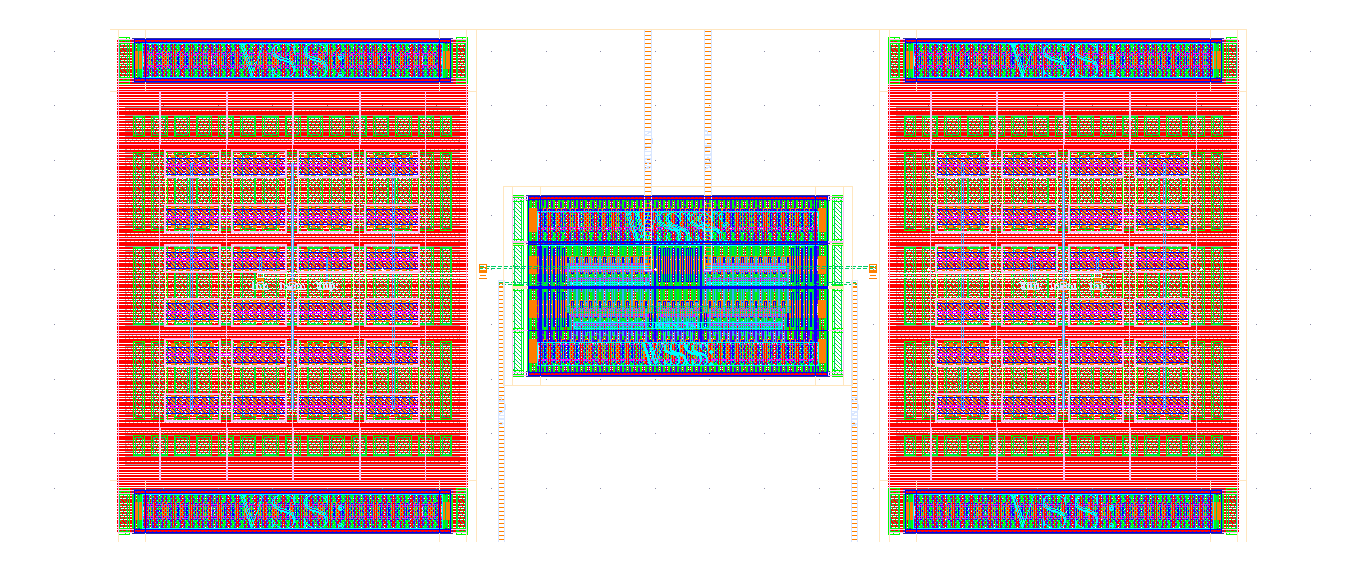
\includegraphics[width=\textwidth]{passive_layout}
  \caption{Full layout}
  \label{fig:sfig1}
\end{subfigure}
\begin{subfigure}{.8\linewidth}
  \centering
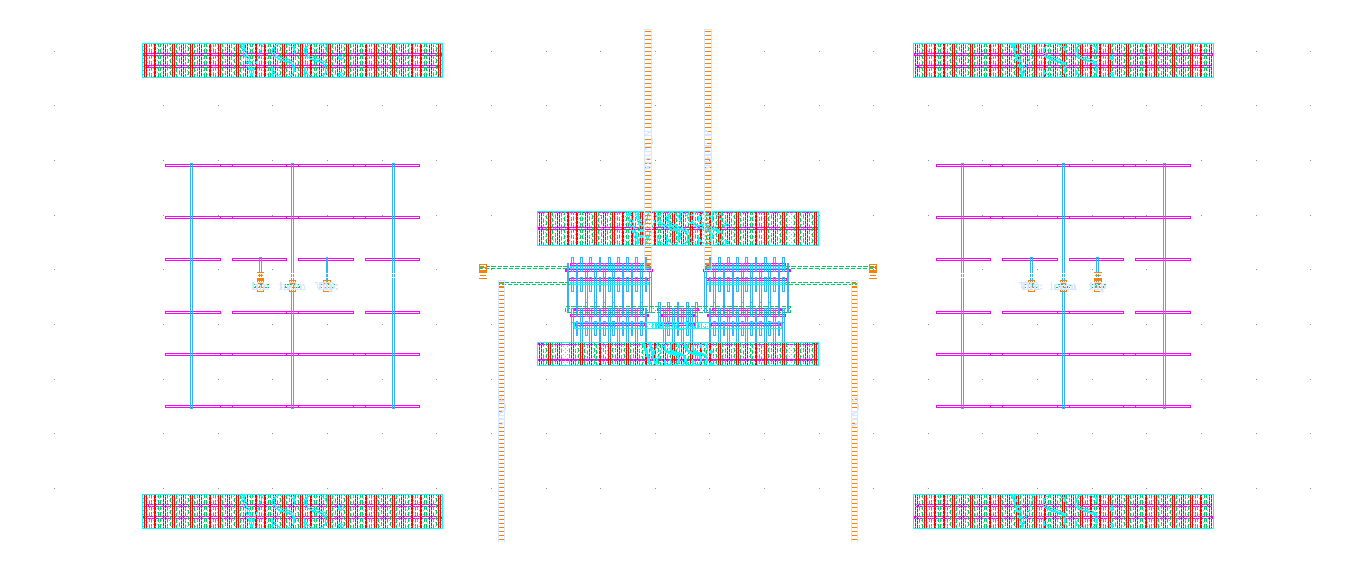
\includegraphics[width=\textwidth]{passive_layout_metals}
  \caption{Only the metals}
  \label{fig:sfig2}
\end{subfigure}
\caption{Differential amplifier layout}
\label{fig:passive_amp}
\end{figure}
All generators demonstrated have wire width parametrized so each type of wire (signal, bias, clock) can have a specific, customizable width. This generator additionally allows the user to specify resistor unit cell sizes, number of parallel and series units and transistor dimensions (width, fingers).

Another option is nearly identical, but with 3-bit resistor DACs instead of a single resistor as in figure \ref{fig:passive_dac}
\begin{figure}[h]
\centering
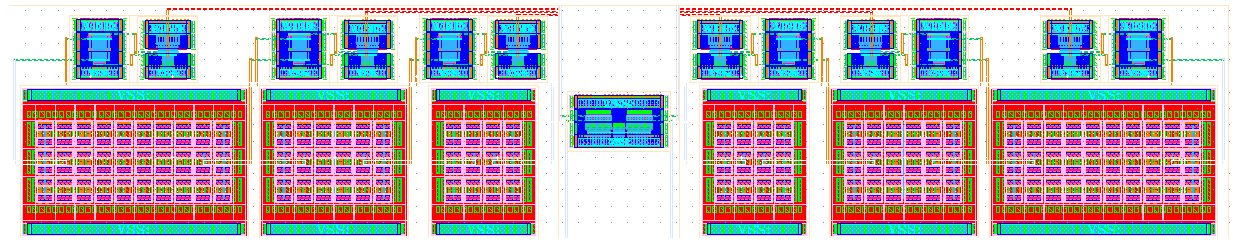
\includegraphics[width=\textwidth]{passive_dac}
\caption{Passive diff-amp with resistor DAC}
\label{fig:passive_dac}
\end{figure}

\section{Getting Fancier: A Double Tail Sense Amplifier and Latch}
Yet another crucial component in an analog receiver is the sampler. Before converting to purely digital processing, the received bits must be processed as either a 1 or a 0 through the use of a sampling circuit. While there are many ways to implement sampling, this report makes use of a double tail sense amp (DTSA). The schematic and operation are shown in Chapter 4. An example layout is shown in figure \ref{fig:dtsa_ex}.
\begin{figure}[h]
\centering
\begin{subfigure}{.4\linewidth}
  \centering
  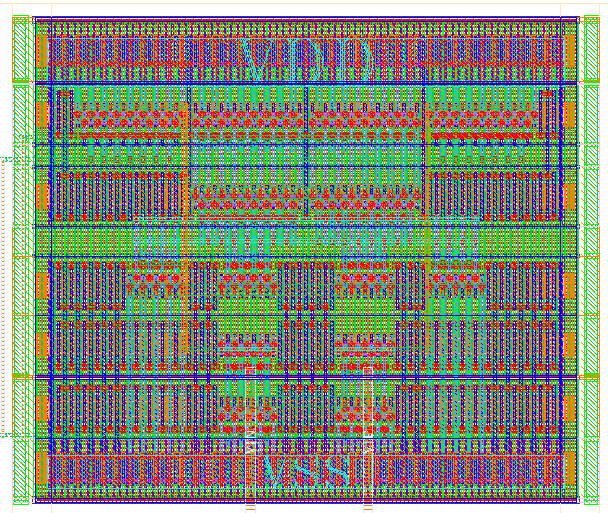
\includegraphics[width=0.8\textwidth]{dtsa_full}
  \caption{Full layout}
  \label{fig:sfig1}
\end{subfigure}
\begin{subfigure}{.4\linewidth}
  \centering
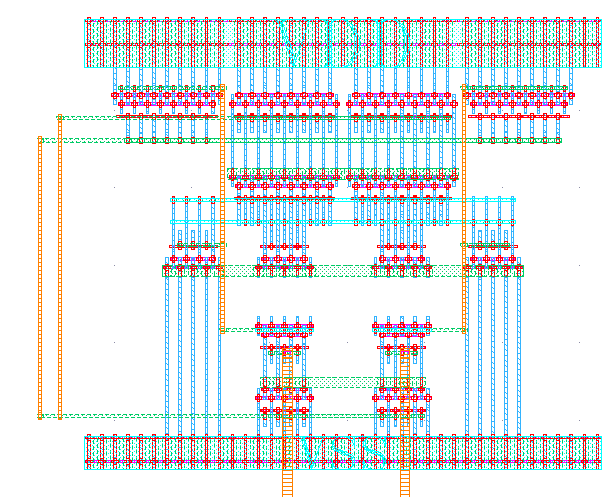
\includegraphics[width=0.8\textwidth]{dtsa_metal}
  \caption{Only the metals}
  \label{fig:sfig2}
\end{subfigure}
\caption{DTSA layout}
\label{fig:dtsa_ex}
\end{figure}
The DTSA block exemplifies even more of BAGs capability to include customization. In addition to all previously mentioned parametrization (wire widths, transistor sizings, etc.) this block also includes an option to generate input pair offset correction hardware. This hardware is implemented as a current that subtracts from the input pair's current during the integration step of operation (discussed more in  Chapter 4). The generator automatically accounts for how the setup changes when offset correction is included and automatically adds more pins/labels to the layout, as shown in figure \ref{fig:dtsa_enoc}.
\begin{figure}[h]
\centering
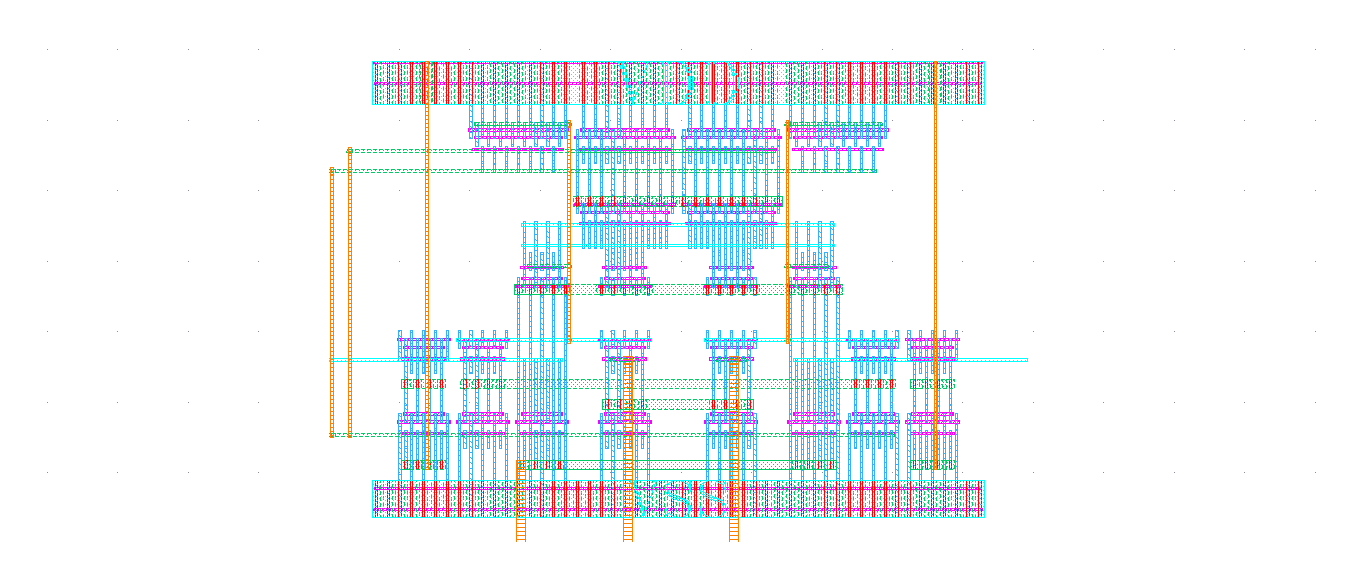
\includegraphics[width=\textwidth]{dtsa_metal_enoc}
\caption{DTSA with offset correction}
\label{fig:dtsa_enoc}
\end{figure}
Finally, the output of a comparator like this is only valid for a short time. We need a latch to store the value in between evaluation cycles. Thankfully, this is possible with BAG. Using TemplateBase we can attach a latch made previously to the output of the DTSA, like in figure \ref{fig:dtsa_d2s}.
\begin{figure}[h]
\centering
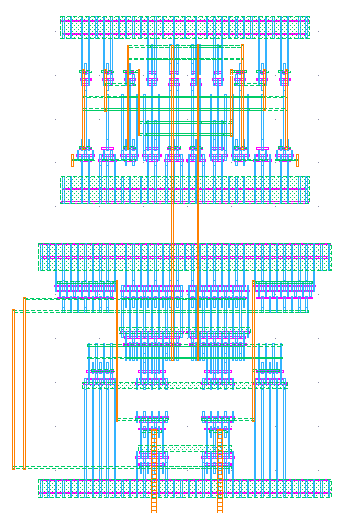
\includegraphics[width=0.4\textwidth]{dtsa_d2s}
\caption{DTSA with latch}
\label{fig:dtsa_d2s}
\end{figure}

\section{Endless Possibilities: An Entire Analog Front End Receiver or Two}
Manually creating the layout for an entire receiver (AFE) is a daunting process. As a final demonstration of how a user can start with small blocks and eventually create large, complex generators, two different front end architectures are shown. It is important to note that the size and complexity of these circuits are non-trivial, and would require significant manual work. These generators are capable of creating and extracting the entire layout in seconds, which truly allows faster design iteration by removing the bottleneck almost entirely. 

The first front end (figure \ref{fig:afe1}) is a chain of a TIA followed by a Cherry-Hooper amplifier stage, then a CTLE and two parallel preamplifiers. 
\begin{figure}[h]
\centering
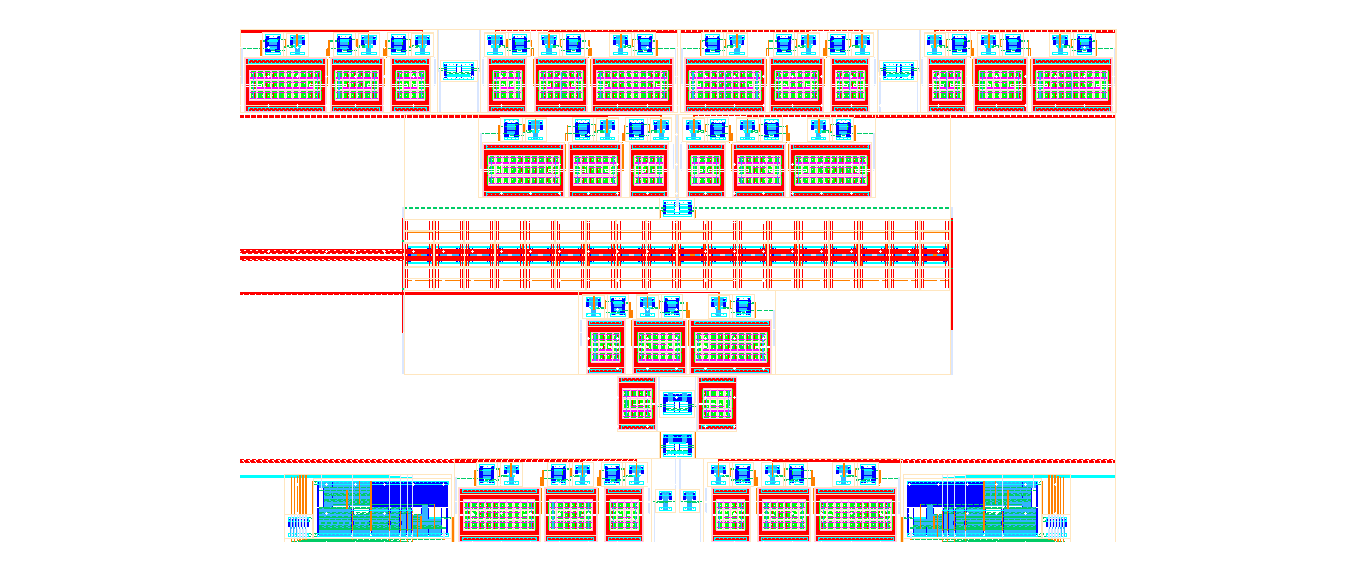
\includegraphics[width=0.3\textwidth]{afe1}
\caption{First front end}
\label{fig:afe1}
\end{figure}
There are also versions that include DACs for every passive element as well as current DACs for every bias input. There are versions that remove the Cherry-Hooper stage and include a comparator. 

Another example of a front end is the one that will be used in Chapter 4. This AFE is a quad data rate AFE similar to the previous AFE and is comprised of the chain: TIA, CTLE, 2x parallel passive diff amps, 4x samplers. The architecture and operation is explained in Chapter 4. The layout is shown in figure \ref{fig:afe2}.
\begin{figure}[h]
\centering
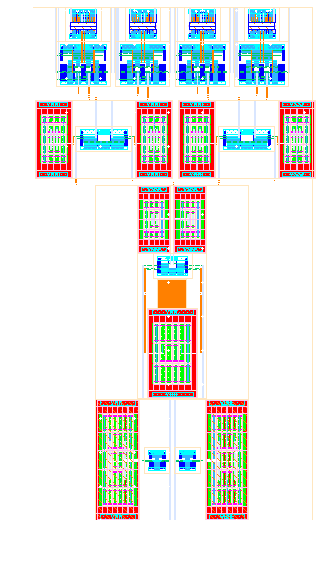
\includegraphics[width=0.3\textwidth]{afe2}
\caption{Second front end}
\label{fig:afe2}
\end{figure}
The main point of demonstrating these layouts is that with a library of ``leaf cells,'' composing large circuits is a very feasible task that would take an experienced user only one to two days to implement. With BAG, layout is no longer a painstaking process.


\chapter{Design Problem: An Optical Receiver}

Photonics is a relatively new field, but the increasing possibility of incorporating photonics elements on chip with the electronics has led to optical circuits becoming a research hotspot. 

To demonstrate the capabilities of BAG, an optical receiver design from concept to verification is shown.

\section{Problem Statement and Architecture}
Photonic communication systems transmit and receive data using light, meaning that the receiver element must be a photo diode. A reverse biased photo diode receiver element can be modeled as a current source with some capacitance in parallel. This is the ``input'', analogous to an antenna in typical RF receivers. For this design, the following arbitrary specs are required:
\begin{itemize}
\item 14nm FinFET technology
\item A data rate of 25Gbps
\item A photo diode capacitance of 50fF
\item $40\mu A$ peak to peak photo diode current
\item $V_{DD}=0.8V$
\item Must use BAG for generation and the majority of testing
\end{itemize}

There are no power constraints or architecture constraints with the condition that any chosen architecture will be implemented in BAG. We will assume the photonics are already implemented, and we will also not simulate for temperature, voltage or process variations. Each transistor will be of a unit size, and only the number of fingers will change. Noise in general should be low, but there is no strict value requirement. We will see in the ``Future Work'' of Chapter 5 how this could be extended, and an example of how one could generalize the design procedure automatically.

\subsection{Architecture Choice and Concerns}
The architecture is based off the receiver in \cite{settaluri_photonic_nodate} and is shown below:
\begin{figure}[h]
\centering
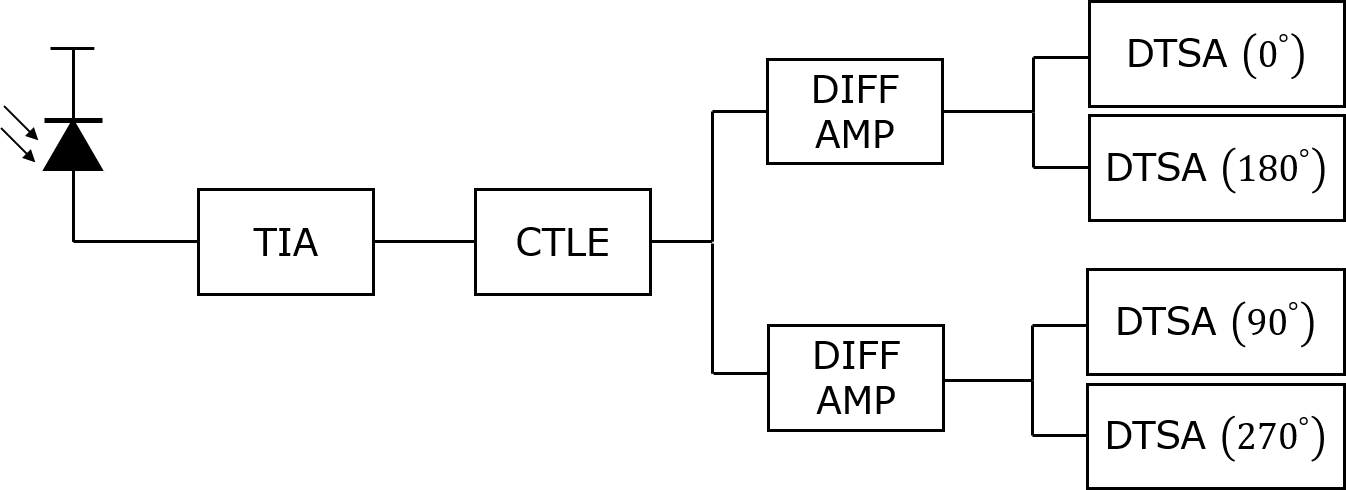
\includegraphics[width=0.7\textwidth]{architecture}
\caption{System architecture}
\label{fig:System Architecture}
\end{figure}

This receiver is a quad data rate (QDR) receiver with each comparator operating in $90^\circ$ phase offsets at a quarter of the clock rate to reduce the comparator constraints. Technically, only a single comparator clocked at 25GHz is necessary, however the time required for a comparator to decide between a 1 or 0 bit is finite, and mostly determined by device limitations rather than designer's choice. To meet the target, we use four comparators that operate only a quarter of the time to allow enough time for decision making and regeneration.This will be further discussed in following parts of this chapter.

Another design choice made is to drive the $0^\circ$ and $180^\circ$ offset comparators with the same preamp, and $90^\circ$and $270^\circ$ together. This was done to reduce the effect of back-injection of the clock into the circuit elements before it.

The transimpedance amplifier (TIA) is the main gain stage and is used to convert the incoming current waveform into a voltage. Since the TIA is the first block in the chain, the formula for cascaded noise figures

\begin{equation}
\label{friis}
F_{total}=F_1+\frac{F_2-1}{G_1}+\frac{F_3-1}{G_1G_2}+...
\end{equation}

(where $F_1$ and $G_i$ are the noise factor and gain of stage $i$ respectively) tells us we want the TIA to be high gain and low noise in order to reduce the overall noise factor of the system.

The TIA is followed by a continuous time linear equalizer (CTLE). A CTLE has a zero in its transfer function that can be placed at a specific frequency, which theoretically allows the designer to extend the bandwidth of previous stages as in figure \ref{fig:CTLE Operation}. One concern of the CTLE however, is that it can only, in general, shape the energy of the frequency spectrum. This means that usually to increase the gain at high frequency, we must throw away DC gain, as shown below:

\begin{figure}[h]
\centering
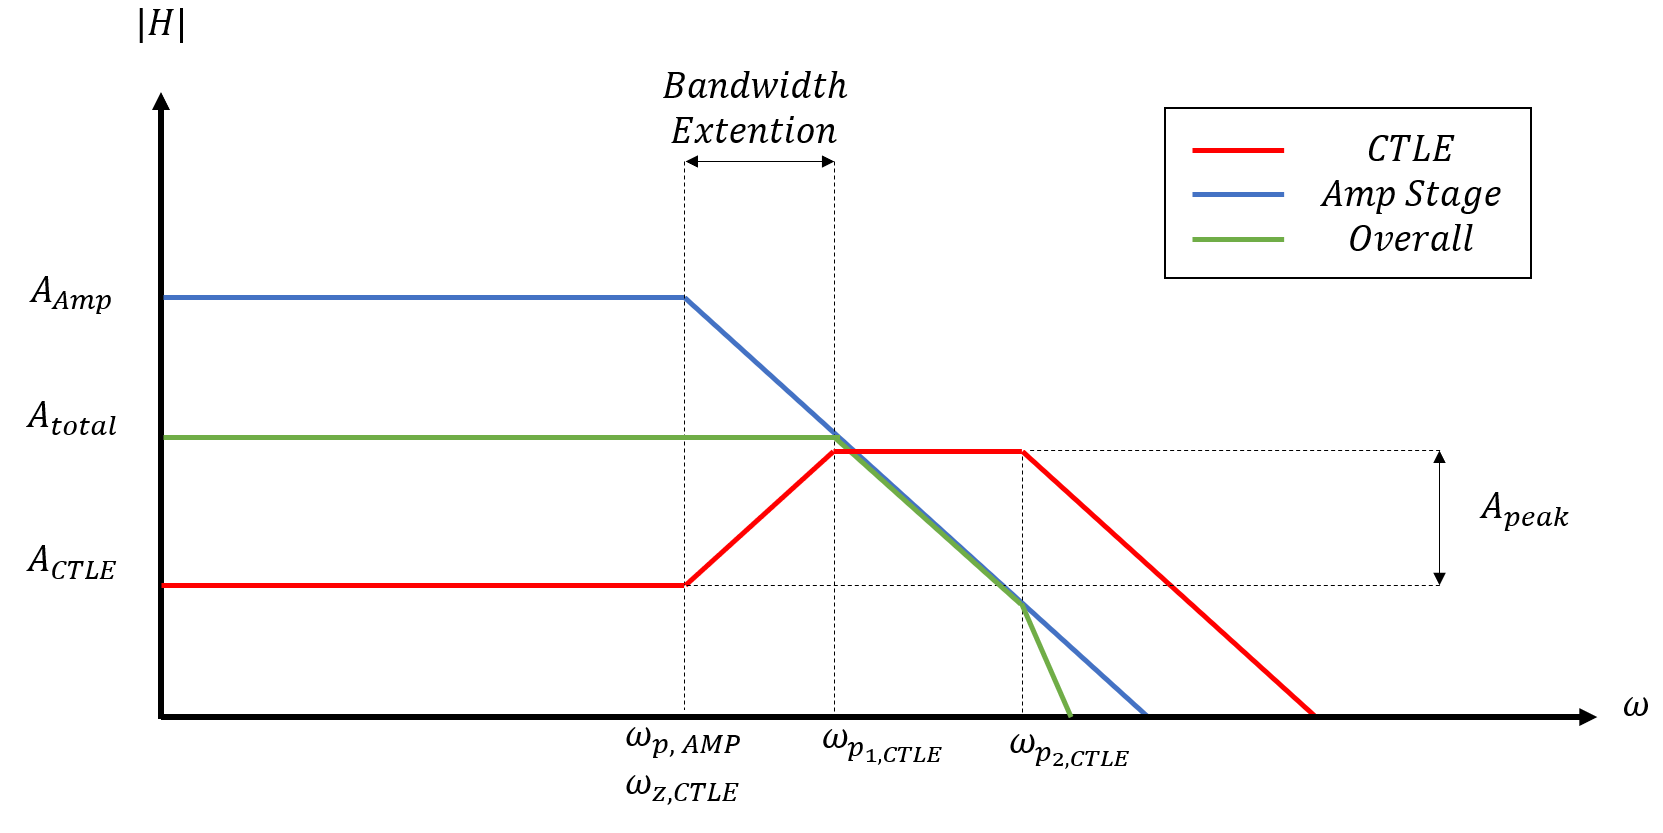
\includegraphics[width=0.8\textwidth]{ctle_operation}
\caption{CTLE effect on a generic one-pole system}
\label{fig:CTLE Operation}
\end{figure}

Since we are targeting 25Gbps, the empirical target bandwidth the front end receiver needs for a relatively optimal trade off in power and introduced ISI is $\approx 0.7\times$ the data rate, or roughly 17GHz \cite{settaluri_first_2017}. The bare minimum would be roughly half, or 12.5GHz. We will target somewhere in between. A good rule of thumb for comparators is that they need milivolts of signal swing to consistently measure correctly. The gain bandwidth product of the TIA is unlikely to be large enough to get a $40\mu A$ signal to roughly $10mV$ across a frequency range of 0Hz to 17GHz and be low noise, so we increase the TIA gain and lower the bandwidth so that even with the CTLE DC gain reduction, we can still get decent gain in conjunction with the CTLE bandwidth extension. 

The final stage before the comparators is a set of passively loaded differential amplifiers. Their purpose is threefold. The CTLE would have to simultaneously drive four comparators, which is a fairly large capacitive load. This limits the maximum achievable peaking gain by pushing in the second pole. Additionally, the comparators tend to inject their clock signal backwards which can impact the CTLE's operation periodically. The amplifiers serve as buffers which will isolate the kickback, and act as an intermediate step to reduce the amount of capacitance the CTLE has to drive. The DC gain is also expected to be too low due to the CTLE's reduction, so the amplifiers will provide a relatively small gain ($\approx 2\times$) to get as much swing as possible.


%\begin{figure}\centering
%\parbox{.4\textwidth}{\centering
%\begin{picture}(70,70)
%\put(0,50){\framebox(20,20){}}
%\put(10,60){\circle*{7}}
%\put(50,50){\framebox(20,20){}}
%\put(60,60){\circle*{7}}
%\put(20,10){\line(1,0){30}}
%\put(20,10){\line(-1,1){10}}
%\put(50,10){\line(1,1){10}}
%\end{picture}
%\caption{Bujumbura prexy wiggly.}}
%\hfill
%\parbox{.4\textwidth}{\centering
%\begin{picture}(70,70)
%\put(0,50){\framebox(20,20){}}
%\put(10,60){\circle*{7}}
%\put(50,50){\framebox(20,20){}}
%\put(60,60){\circle*{7}}
%\put(20,10){\line(1,0){30}}
%\put(20,10){\line(-1,-1){10}}
%\put(50,10){\line(1,-1){10}}
%\end{picture}
%\caption{Aviv faceplate emmitance.}}
%\end{figure}

\section{Transimpedance Amplifier}
The TIA is implemented as a pseudo-differential structure as two CMOS inverters with resistive feedback. 
\begin{figure}[h]
\centering
\ctikzset{tripoles/mos style/arrows}
\begin{circuitikz}[american voltages]
\draw (3, 2) node[american not port](n){};
\draw (3, 3.5) node[american not port](p){};
\draw (p.out) to[short] (4, 3.5) |- (4, 4.5) to[R, l_=$R_{fb}$] (2, 4.5);
\draw (p.in) -| (2, 4.5);
\draw (n.out) to[short] (4, 2) |- (4, 1) to[R, l=$R_{fb}$] (2, 1);
\draw (n.in) -| (2, 1);
\draw (p.out) to[short, -o] (5, 3.5) to[open, v^=$V_{out}$, -o] (5, 2) to[short] (n.out);
\draw (p.in) to[short] (-1, 3.5) to[american current source, l_=$I_{DC}$] (-1, 2) to[short] (-1, 1.5) node[ground]{};
\draw (-1, 3.5) to[short, *-] (-1, 4) to[pDo] (-1, 4.5) to[short] (-1, 5) node[rground, yscale=-1]{} to[open] (-1, 5.5) node[above]{$V_{DD}$};
\draw (-1, 4.75) to[short] (0, 4.75) to[C, l=$C_{pd}$] (0, 3.5);
\draw (n.in) to[short] (1, 2) to[american current source, l_=$I_{DC}$] (1, 0.5) to[short] (1, 0) node[ground]{};
\end{circuitikz}
\label{TIA Schematic}
\caption{TIA Schematic}
\end{figure}

The purpose of implementing the TIA is due to the usage in both \cite{mehta_12gb/s_2016} and \cite{settaluri_photonic_nodate}. The photodetector can split into a differential input that achieves good performance. At DC, if $I_{DC}=0$ then the input and output common mode voltages are equal. The purpose of the DC current source is to force the output common mode to be higher if desired. Since the output will sit about mid-rail, that may not be enough to bias the input of the CTLE, so we will need DC current through $R_{fb}$ to force this difference.

If we assume the inverters are an amplifier with gain $-A_v$ then the input impedance can be found by using Miller's theorem. 
\begin{equation}
\label{TIA input impedance}
Z_{in}=Z_{C_{pd}}||(1+A_v)R_{fb}
\end{equation}
which simplifies to 
\begin{equation}
\label{TIA input impedance}
\frac{(1+A_v)R_{fb}}{1+j\omega (1+A_v)C_{pd}R_{fb}}
\end{equation}
Thus the input pole should be roughly at
\begin{equation}
\label{TIA input pole}
\omega_p=\frac{1}{(1+A_v)R_{fb}C_{pd}}
\end{equation}

\begin{figure}[h]
\centering
\ctikzset{tripoles/mos style/arrows}
\begin{circuitikz}[american voltages]
\draw (0, 0) to[american current source, v=$v_{gs}$, l=$i_{in}$] (0, 2.5);
\draw (0, 0) node[ground]{};
\draw (0, 2.5) to[R, l=$R_{fb}$] (2, 2.5);
\draw (2, 2.5) to[american controlled current source, l=$g_{mn} v_{gs}$] (2, 0);
\draw (2, 2.5) to[short] (4.5, 2.5) to[american controlled current source, l=$g_{mp} v_{gs}$] (4.5, 0);
\draw (4.5, 2.5) to[short] (7, 2.5) to[R, l=$r_{on}||r_{op}$] (7, 0);
\draw (7, 2.5) to[short, -o] (8, 2.5) node[label={[font=\footnotesize]0:$v_{out}$}] {};
\draw (7, 0) to[short] (0, 0);
\end{circuitikz}
\caption{TIA Small Signal Model}
\label{fig:PLEASE}
\end{figure}
From the small signal model of one half of the circuit (shown in figure \ref{fig:PLEASE}, ignoring $C_{pd}$) we can derive the gain. KCL at the output node gives
\begin{equation}
\label{TIA gain KCL}
\frac{v_{out}}{r_{on}||r_{op}}+(g_{mn}+g_{mp})(i_{in}R_{fb}+v_{out})-i_{in}=0
\end{equation}
which simplifies to
\begin{equation}
\label{TIA gain full}
\frac{v_{out}}{i_{in}}=\frac{R_{fb}(g_{mn}+g_{mp})-1}{-(g_{mn}+g_{mp})-\frac{1}{r_{on}||r_{op}}}
\end{equation}
If we assume $R_{fb}$ and $r_{on}||r_{op}$ are both much larger than 1, then the transfer function simplifies to
\begin{equation}
\label{TIA gain}
|\frac{v_{out}}{i_{in}}|=R_{fb}
\end{equation}
The gain is then approximately just $R_{fb}$. For a given choice of $R_{fb}$, we then use BAGs rapid iteration to sweep for transistor widths. As the size increases, device parasitics become dominant over the external capacitances, so there is an optimal size for bandwidth. Once the maximum bandwidth is found, this sets the device sizes. Since we know the CTLE can only get a couple of GHz of bandwidth extension, we can calculate and then sweep the TIA resistor to see what resistance gives a bandwidth of around 9GHz. If we assume the CTLE will cut the DC gain by roughly a third, and we can get about 1.5x amplification from the preamps, then the overall gain should still be high enough for the comparator.

To set the output common mode, we can assume the input will be around mid-rail, so the output can be approximated as follows:
\begin{equation}
\label{tia_dc}
\frac{V_{o}-\frac{V_{DD}}{2}}{R_{fb}}=I_{DC}
\end{equation}
In order to bias the CTLE input, we want this to potentially be a little higher than midrail since the $V_{GS}$ needs to be large enough to give headroom to the tail transistors. Plugging into equation \ref{tia_dc} gives a starting point that can then be swept using BAG for better accuracy. Post-PEX hand-simulation is then used to fine tune the current the get the desired result. Note that by increasing the output common mode, the gain can reduce. This means that the resistance might need to be higher than anticipated. This is also determined by simulating BAG generated instances.

We were able to achieve a gain of 1500 with a bandwidth of 8.55GHz. In order to shift the common mode, $I_{DC}$ was set to $55\mu A$.

\section{Continuous Time Linear Equalizer}
A CTLE is a simple amplifier, degenerated by a parallel resistor capacitor combination as shown below:
\begin{figure}[h]
\centering
\ctikzset{tripoles/mos style/arrows}
\begin{circuitikz}[american voltages]
\draw (1, 1) node[nmos](n_in){};
\draw (3, 1) node[nmos, xscale=-1](p_in){};
\draw (n_in.drain) to[R, l=$R_d$] (1, 3.5);
\draw (1, 3.5) to[short] (2, 3.5) node[above]{$V_{DD}$};
\draw (2, 3.5) to[short] (3, 3.5) to[R, l=$R_d$] (p_in.drain);
\draw (n_in.source) to[C, *-,  l=$C_s$] (p_in.source);
\draw (n_in.source) to[short] (1, -1) to[R, *-*, l=$R_s$] (3, -1) to[short, -*] (p_in.source);
\draw (1, -2) node[nmos](n_tail){};
\draw (n_tail.drain) to[short] (1, -1);
\draw (3, -2) node[nmos](p_tail){};
\draw (p_tail.drain) to[short] (3, -1);
\draw (n_tail.source) to[short] (1, -3) to[short, -*] (2, -3) node[ground]{};
\draw (2, -3) to[short] (3, -3) to[short] (p_tail.source);
\draw (-1, -2) node[nmos, xscale=-1](bias){};
\draw (bias.source) to[short] (-1, -3) to[short] (2, -3);
\draw (bias.drain) to[short, -o] (-1, 0) node[above]{$I_{bias}$};
\draw (-1, -1) to[short, *-] (0, -1) to[short, -*] (bias.gate);
\draw (bias.gate) to[short] (p_tail.gate);
\draw (n_in.gate) node[label={[font=\footnotesize]180:$V_{in}$}] {};
\draw (p_in.gate) node[label={[font=\footnotesize]0:$V_{ip}$}] {};
\draw (p_in.drain) to[short, -o] (2.5, 1.77) to[open, v=$V_{out}$] (1.5, 1.77) to[short, o-] (n_in.drain);
\end{circuitikz}
\label{CTLE Schematic}
\caption{CTLE Schematic}
\end{figure}

Since we know the pole location of the TIA after simulation, we can design the CTLE to have its zero in close proximity. Firstly, we draw the approximate differential mode half circuit:

\begin{figure}[h]
\centering
\ctikzset{tripoles/mos style/arrows}
\begin{circuitikz}[american voltages]
\draw (1, 1) node[nmos](n_in){};
\draw (n_in.drain) to[R, l=$R_d$] (1, 3.5);
\draw (1, 3.5) node[rground, yscale=-1]{} to[open] (1, 4) node[above]{$V_{DD}$};
\draw (n_in.source) to[short] (1, 0) to[short] (0.5, 0) to[R, l_=$\frac{R_s}{2}$] (0.5, -1.5);
\draw (n_in.source) to[short] (1, 0) to[short] (1.5, 0) to[C, l=$2C_s$] (1.5, -1.5);
\draw (1.5, -1.5) to[short, -*] (1, -1.5) to[short] (0.5, -1.5);
\draw (1, -1.5) node[ground]{};
\draw (n_in.drain) to[short, -o] (1.5, 1.77)  node[label={[font=\footnotesize]0:$V_{out}$}] {};
\draw (n_in.gate) node[label={[font=\footnotesize]180:$V_{in}$}] {};
\end{circuitikz}
\label{CTLE Half-Circuit}
\caption{CTLE Half-Circuit}
\end{figure}

which by inspection, we know
\begin{equation}
\label{Gm}
G_m=\frac{g_m}{1+g_m(\frac{R_s}{2}||\frac{Z_{C_s}}{2})}
\end{equation}
\begin{equation}
G_m=\frac{2g_m(1+j\omega R_sC_s)}{2+g_mR_s+2j\omega R_sC_s}
\end{equation}
We can also determine the output impedance by inspection
\begin{equation}
\label{Ro}
R_o\approx R_l||\frac{Z_{C_l}}{2}=\frac{R_d}{1+2j\omega R_d C_l}
\end{equation}
So the overall gain is then
\begin{equation}
\label{ctle_gain}
G_mR_o=\frac{2g_m(1+j\omega R_sC_s)R_d}{(2+g_m R_s+2j\omega R_sC_s)(1+2j\omega R_dC_l)}
\end{equation}
which puts the zero at 
\begin{equation}
\label{zero}
\omega_z=\frac{1}{R_sC_s}
\end{equation}
and the first pole at 
\begin{equation}
\label{pole_1}
\omega_{p1}=\frac{1+gm\frac{R_s}{2}}{R_sC_s}
\end{equation}
with the second pole at
\begin{equation}
\label{pole_2}
\omega_{p2}=\frac{1}{2R_dC_l}
\end{equation}
and lastly, the ideal peaking gain should be 
\begin{equation}
\label{peak gain}
A_{peak}=g_mR_d
\end{equation}
From these equations, we can choose the values of the degeneration components and pullup resistors to place the zero and set the peak gain. We want the second pole to be far away at roughly 20GHz or more, which fixes $R_d$ for a given $C_l$. If we want a peak gain of around 2, that then fixes the required $g_m$, which for an assumed $V_{ov}$ of 200mV, fixes the bias current and transistor sizes. We will (quite conservatively) assume the input to each amplifier is 10fF, so the total load is 20fF. Through BAG, we can sweep component values near the desired points to get more accurate results.

Using the above steps, we were able to achieve a bandwidth extension of about 4GHz with a DC gain of roughly 0.6. When placed in succession to the TIA, the overall gain reduces to about 850 with a bandwidth extension to about 13.5GHz.

\section{Preamplifiers}
The preamplifiers are implemented as passively-loaded differential amplifiers as shown below. The main purpose is to serve as a buffer between the CTLE and the DTSAs. The DTSAs will provide a fairly substantial capacitive load to the CTLE as well as back-inject their clock, which is undesired. The preamplifiers ideally will have a gain of around 2, but we will target a gain greater than 1. 

\begin{figure}[h]
\centering
\ctikzset{tripoles/mos style/arrows}
\begin{circuitikz}[american voltages]
\draw (1, 1) node[nmos](n_in){};
\draw (3, 1) node[nmos, xscale=-1](p_in){};
\draw (n_in.drain) to[R, l=$R_d$] (1, 3.5);
\draw (1, 3.5) to[short] (2, 3.5) node[above]{$V_{DD}$};
\draw (2, 3.5) to[short] (3, 3.5) to[R, l=$R_d$] (p_in.drain);
\draw (n_in.source) to[short] (1, 0) to[short, *-*] (3, 0) to[short] (p_in.source);
\draw (1, -1) node[nmos](n_tail){};
\draw (n_tail.drain) to[short] (1, 0);
\draw (3, -1) node[nmos](p_tail){};
\draw (p_tail.drain) to[short] (3, 0);
\draw (n_tail.source) to[short] (1, -2) to[short, -*] (2, -2) node[ground]{};
\draw (2, -2) to[short] (3, -2) to[short] (p_tail.source);
\draw (-1, -1) node[nmos, xscale=-1](bias){};
\draw (bias.source) to[short] (-1, -2) to[short] (2, -2);
\draw (bias.drain) to[short, -o] (-1, 0.5) node[left]{$I_{bias}$};
\draw (-1, 0) to[short, *-] (0, 0) to[short, -*] (bias.gate);
\draw (bias.gate) to[short] (p_tail.gate);
\draw (n_in.gate) node[label={[font=\footnotesize]180:$V_{in}$}] {};
\draw (p_in.gate) node[label={[font=\footnotesize]0:$V_{ip}$}] {};
\draw (p_in.drain) to[short, -o] (2.5, 1.77) to[open, v=$V_{out}$] (1.5, 1.77) to[short, o-] (n_in.drain);
\end{circuitikz}
\label{fig:preamp_schematic}
\caption{Preamp Schematic}
\end{figure}

Assuming the $r_o$ of the transistors are fairly large, then the gain of this amplifier is known to be
\begin{equation}
\label{preamp gain}
A_v=g_mR_d
\end{equation}
with the unity gain frequency at
\begin{equation}
\label{preamp ugb}
\omega_u=\frac{g_m}{C_l}
\end{equation}
Once we know the bandwidth of the CTLE, we can determine the required unity gain bandwidth for an overall gain of 2 at this frequency. Again assuming each DTSA provides 10fF of load, then we know $C_l$. This fixes the required $g_m$ and therefore the device sizes and bias current.

Following these steps, the amplifiers were able to obtain a gain of 1.5 up to 13.5GHz. This sets the entire front end chain to have an overall bandwidth of 13.5GHz and a gain of 1200. Assuming a $40\mu A$ peak-to-peak input current swing, this should be plenty for the comparator.

\section{Comparator}

The comparator is implemented as a double tail sense amplifier. 
\begin{figure}[h]
\centering
\ctikzset{tripoles/mos style/arrows}
\begin{circuitikz}[american voltages]
\draw (0, 0) node[nmos](tail_left){};
\draw (2, 0) node[nmos, xscale=-1](tail_right){};
\draw (tail_left.gate) node[label={[font=\footnotesize]180:$CLK$}] {};
\draw (tail_right.gate) node[label={[font=\footnotesize]0:$CLK$}] {};
\draw (tail_left.source) to[short] (0, -1) to[short, -*] (1, -1) node[ground]{} to[short] (2,-1) to[short] (tail_right.source);
\draw (0, 2) node[nmos](in_left){};
\draw (2, 2) node[nmos, xscale=-1](in_right){};
\draw (in_left.gate) node[label={[font=\footnotesize]180:$V_{in}$}] {};
\draw (in_right.gate) node[label={[font=\footnotesize]0:$V_{ip}$}] {};
\draw (in_left.source) to[short, -*] (tail_left.drain) to[short] (tail_right.drain) to[short, *-] (in_right.source);
\draw (0, 4) node[pmos, xscale=-1](left_reset){};
\draw (2, 4) node[pmos](right_reset){};
\draw (right_reset.gate) node[label={[font=\footnotesize]90:$CLK$}] {};
\draw (left_reset.gate) to[short] (right_reset.gate);
\draw (left_reset.drain) to[short, l=$D_{ip}$, -*] (in_left.drain);
\draw (right_reset.drain) to[short, l_=$D_{in}$, -*] (in_right.drain);
\draw (left_reset.source) to[short, l=$V_{DD}$] (right_reset.source);
\draw (-3, 8) node[nmos](left_switch){};
\draw (-1, 8) node[nmos, xscale=-1](inv_left_n){};
\draw (3, 8) node[nmos](inv_right_n){};
\draw (5, 8) node[nmos, xscale=-1](right_switch){}; 
\draw (-1, 10) node[pmos, xscale=-1](inv_left_p){};
\draw (-1, 12) node[pmos](p_switch_left){};
\draw (3, 10) node[pmos](inv_right_p){};
\draw (3, 12) node[pmos, xscale=-1](p_switch_right){};
\draw (in_left.drain) to[short] (-4, 2.77) to[short] (left_switch.gate);
\draw (in_right.drain) to[short] (6, 2.77) to[short] (right_switch.gate);
\draw (left_switch.source) to[short, -*] (inv_left_n.source) to[short, -*] (1, 7.23) to[short, -*] (inv_right_n.source) to[short] (right_switch.source);
\draw (1, 7.23) node[ground]{};
\draw (left_switch.drain) to[short, l=$V_{on}$] (inv_left_n.drain);
\draw (right_switch.drain) to[short, l_=$V_{op}$] (inv_right_n.drain);
\draw (inv_left_n.drain) to[short] (inv_left_p.drain);
\draw (inv_right_n.drain) to[short] (inv_right_p.drain);
\draw (inv_left_p.gate) to[short] (inv_left_n.gate);
\draw (inv_right_p.gate) to[short] (inv_right_n.gate);
\draw (inv_left_n.drain) to[short, *-*] (2.025, 8.77);
\draw (inv_right_p.drain) to[short, *-*] (-0.025, 9.225);
\draw (inv_left_p.source) to[short] (p_switch_left.drain);
\draw (inv_right_p.source) to[short] (p_switch_right.drain);
\draw (p_switch_left.source) to[short, l=$V_{DD}$] (p_switch_right.source);
\draw (p_switch_left.drain) to[short, *-*] (p_switch_right.drain);
\draw (p_switch_left.gate) node[label={[font=\footnotesize]180:$\overline{CLK}$}] {};
\draw (p_switch_right.gate) node[label={[font=\footnotesize]0:$\overline{CLK}$}] {};
\end{circuitikz}
\label{Double Tail Schematic}
\caption{Double Tail Schematic}
\end{figure}
\clearpage
The DTSA consists of a clocked differential pair that feeds into cross-coupled inverters. Much like the classic StrongArm sense-amp \cite{razavi_strongarm_2015}, the DTSA first precharges the $D_{in}$ and $D_{ip}$ nodes up to $V_{DD}$. After $CLK$ goes high, the input pairs activate and begin to drain charge from the parasitic capacitance at nodes $D_{in}$ and $D_{ip}$. Depending on which input is larger, one side will discharge faster which will turn off one of the switches connected to those nodes faster than the other. This sets the value in the cross-coupled inverters which is then reinforced through positive feedback. 

When $CLK$ goes low, the circuit resets and precharges the $D_{ip}/D_{in}$ nodes for the next cycle.

A typical cycle of the DTSA with a differential input of 10mV is plotted in figure \ref{fig:dtsa_op}. The clock is generated by taking ideal clocks and passing them through a chain of inverters to generate both the real $CLK$ and $\overline{CLK}$ signals.
\begin{figure}[h]
\centering
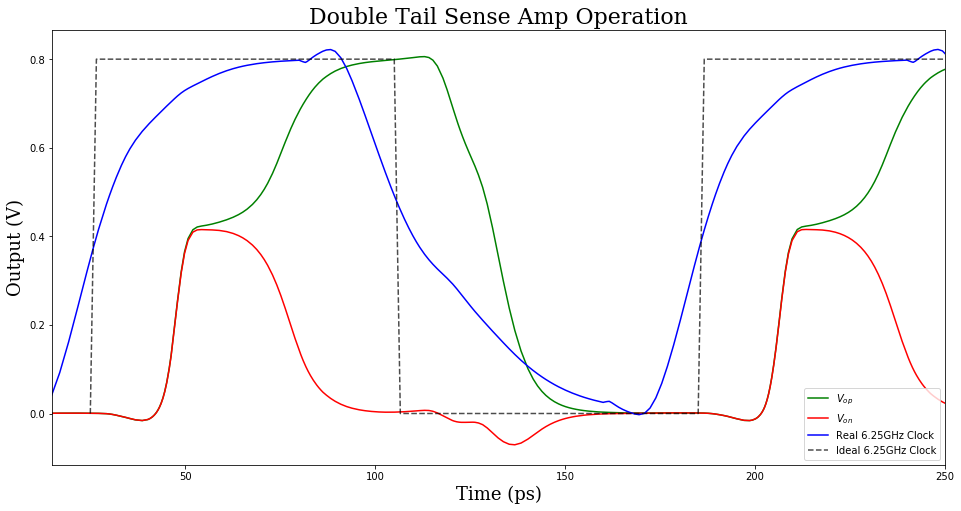
\includegraphics[width=\textwidth]{dtsa_one_cycle}
\caption{DTSA Typical Operation}
\label{fig:dtsa_op}
\end{figure}

The comparator usually is the first thing one would design, as its limitations generally set the required gain and noise specs for the front end. In this project, the comparator was designed last, since there is no power constraint. The rate at which voltage is reduced from $D_{ip}/D_{in}$ is based on the current through the input pairs. By increasing the size of the input pairs, we can create a voltage difference much more quickly (assuming there is no process offset in the input pairs) which allows even small inputs to be sensed before the cycle ends. Thus, as long as our input is on the order of milivolts, we should be able to sense this.

As a test, we determine what the approximate noise tolerance of the DTSA is. We input a small differential signal (about 1mV) and run a transient simulation with noise over many cycles. The fraction of incorrect evaluations to the total allows us to approximate $\sigma_n$, or the standard deviation of the noise tolerance for the DTSA. The results of this simulation are shown in figure \ref{fig:dtsa_noise}.
\begin{figure}[h]
\centering
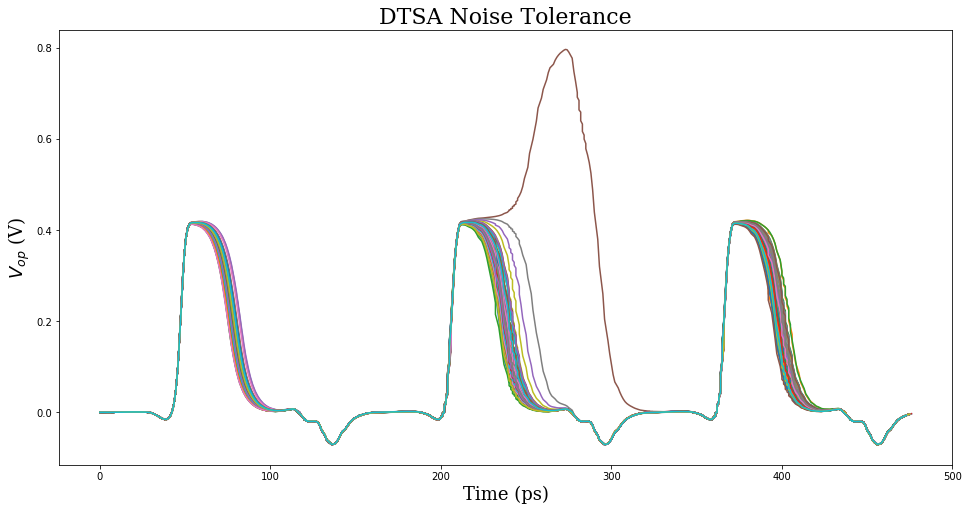
\includegraphics[width=\textwidth]{dtsa_noise_tolerance}
\caption{DTSA Noise}
\label{fig:dtsa_noise}
\end{figure}
With a differential input of 1mV, only one in 100 inputs failed. This implies two things. One, that 1mV is approximately $3\sigma_n$. This means we should budget about 3mV of the eye opening to noise tolerance for the DTSA for a BER of $10^{-12}$. Secondly, the DTSA minimum input voltage is less than 1mV, assuming no noise. Thus, as long as our input has a swing of 1mV in addition to the noise budget, then we should be able to obtain a bit error rate of $10^{-12}$. This, of course, ignores process variation. Process variation introduces an offset that affects the current in each branch. From a Monte Carlo simulation, one can find the average offset which can then additionally be added to the eye opening budget. There are also topologies that can correct for offset, which would not completely eliminate the issue, but would certainly reduce it.
\clearpage
\section{Design Verification}
There were four simulations done to verify the behavior of the entire receiver. Firstly, a simple AC simulation of the front-end chain up to the samplers in order to see if the circuit provides enough gain. This is shown in figure \ref{fig:afe_ac}
\begin{figure}[h]
\centering
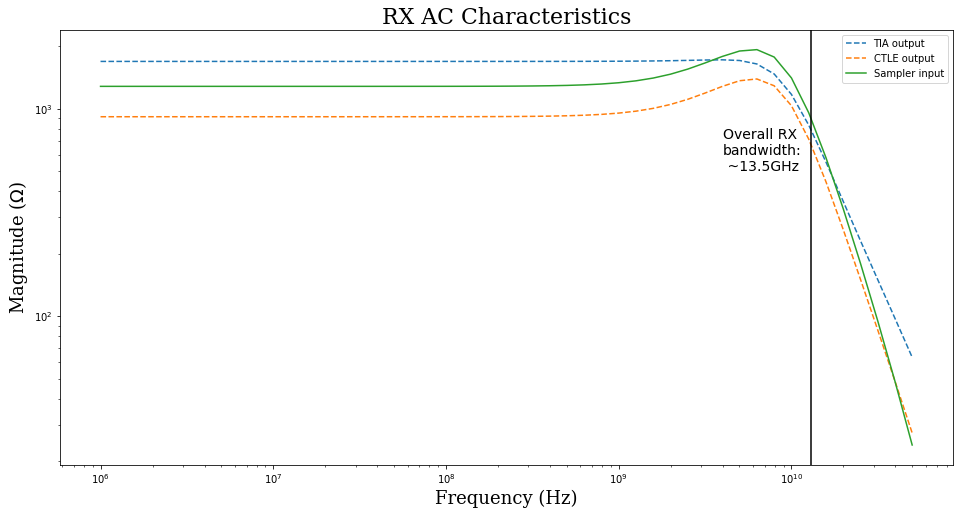
\includegraphics[width=\textwidth]{rx_ac_char}
\caption{AFE AC Performance}
\label{fig:afe_ac}
\end{figure}
\clearpage
To determine how much noise the amplifier chain introduces, an AC noise simulation was also run. The power spectral density is plotted in figure \ref{fig:psd}.
\begin{figure}[h]
\centering
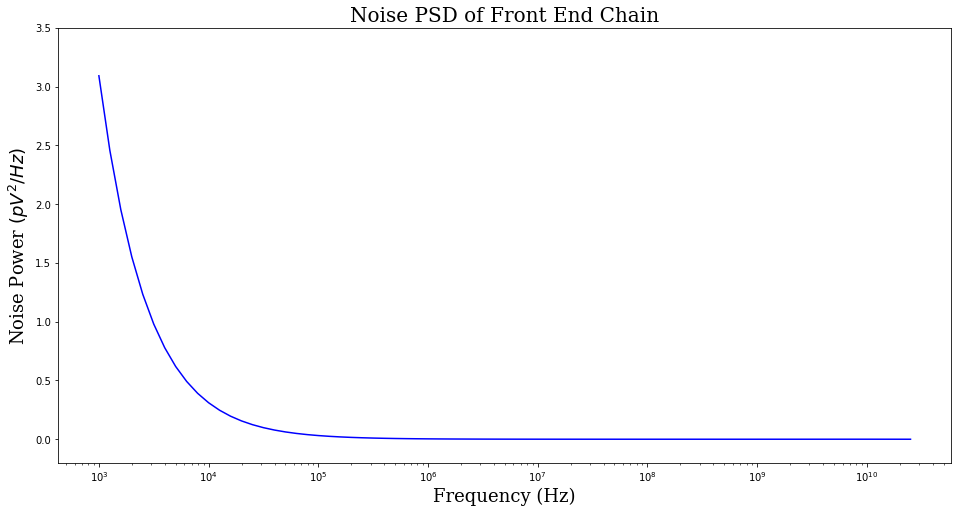
\includegraphics[width=\textwidth]{ac_noise}
\caption{Front End Noise PSD}
\label{fig:psd}
\end{figure}

Using Python to integrate this function up to 25GHz gives an rms noise of $4.6\mu V^2$, so the mean expected noise is then 2mV.
\clearpage
From the previous sections, we know that the minimum input is approximately 1mV with a noise tolerance of 3mV for a BER of $10^{-12}$. For an input of $40\mu A$ peak-to-peak, we achieve a gain of 1200 which puts the input amplitude at roughly 50mV peak-to-peak. This should be plenty. Unfortunately, the desired bandwidth was not met, although the bandwidth does surpass the theoretical minimum. This will mostly affect ISI performance, which will be seen in the next simulation.

To determine over many cycles how the AFE performs, we measure the eye diagram at the sampler inputs. This is shown in figure \ref{fig:eye}.
\begin{figure}[h]
\centering
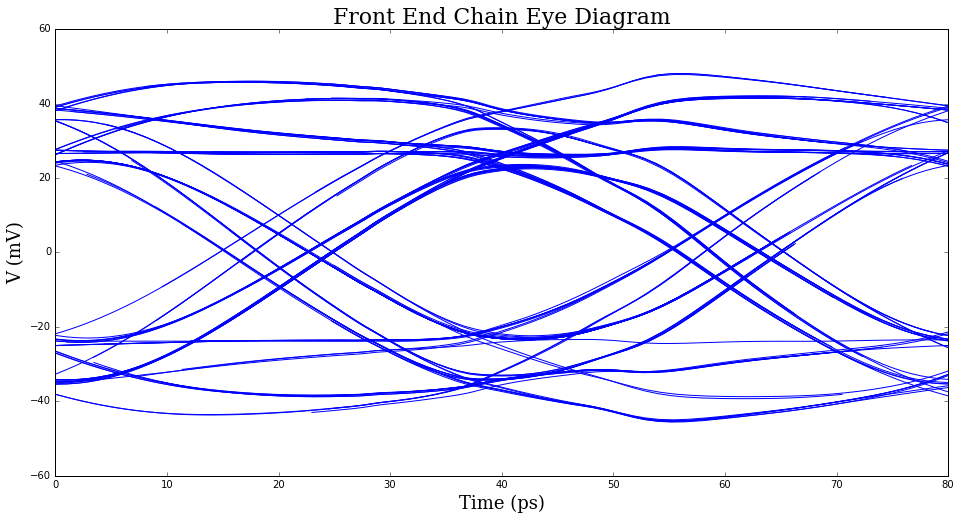
\includegraphics[width=\textwidth]{afe_eye}
\caption{Sampler Input Eye Diagram}
\label{fig:eye}
\end{figure}
As can be seen, there is a fairly large eye opening which surpasses the minimum required swing for proper evaluation.
\clearpage
Lastly, a PRBS32 pattern is fed into the receiver, and the sampler outputs are monitored in a transient simulation. Note that this architecture would not operate sufficiently due to the fact that the waveforms need to be adjusted in time to center the eye opening with the clock edges. This adjustment was done manually for this test. Also, since each sampler is only sampling once every 4 bits, the outputs are sliced and manually stitched together. A portion of the test input and output are shown in figure \ref{fig:prbs}. The patterns are clearly identical with only a time offset through the front end chain.
\begin{figure}[h]
\centering
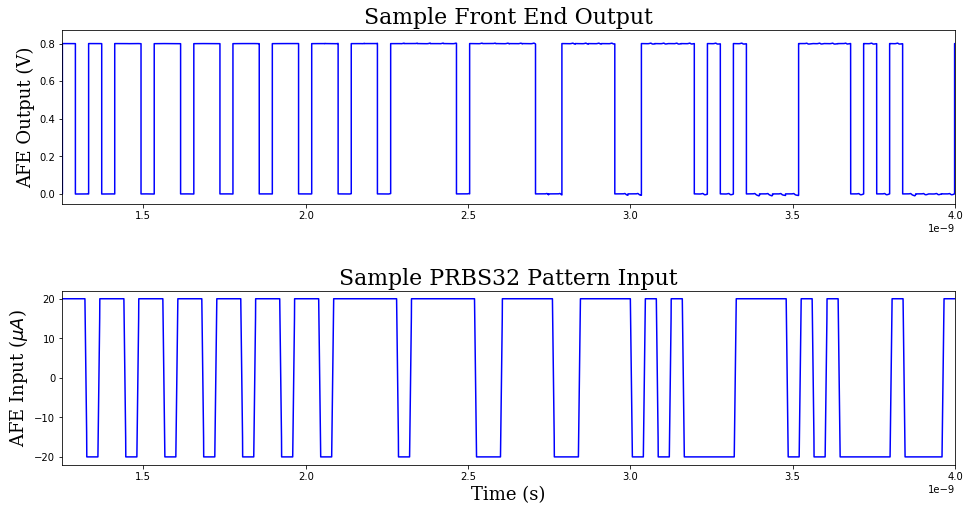
\includegraphics[width=\textwidth]{prbs_out}
\caption{PRBS Pattern Response}
\label{fig:prbs}
\end{figure}
\clearpage

\chapter{Conclusions, Future Work and Other Possibilities}
And here we are at the finale. For those who made it this far, congrats! To those who read only the abstract before this, welcome. I hope it's interesting!
\section{How BAG Saved the Day}
A good question to ask is how BAG improved the process, if at all? The classic strategy would be to design with only some regard to layout parasitics, and simply hope the effect is not too great. Should the effects prove to be too substantial, modify the design and iterate until a solution is found. Does BAG fix this problem? The generators had to be written first which is clearly a non-trivial task. What time is even saved? What is the benefit over the old way? 

Writing a generator is indeed a non-trivial task, however it only needs to be done once. A well-written generator will take any inputs (within reason) and generate a verified circuit with layout in seconds. An experienced BAG user can plausibly create a complicated generator in one to two days, which essentially permanently removes layout from the design iteration. Rather than spend two days on layout each time a change is made, a large time investment is made upfront for massive time savings in the future. BAG truly allows a designer to close the analog loop faster by removing the bottleneck from layout. If a user was provided a library of generators, the time savings are even greater. With a set of verified generators, the guesswork is completely taken out of the design process. Previously, parasitics either had to be estimated or ignored, and then accounted for afterwards. Now, parasitics can be directly included since the layout is essentially ``free.'' 

With BAG, the author was able to design, generate and (partially) test a fully LVS/PEX verified receiver front end working part-time in roughly two weeks. With an architecture chosen, only the sizing remained. Since layout generation was not an issue, seeing the effects of parasitics simplified the design process since they could be included automatically. Using \texttt{SweepDesignManager} mentioned in Chapter 3, it becomes very easy to fine-tune parameters through sweeping automatically, since BAG will run PEX/LVS and simulate many designs in parallel. This way, the trade offs between component value choices are very clear and quick to see. Furthermore, no one had to painstakingly draw the layout by hand, massively improving life quality.
%\begin{figure}\centering
%\parbox{.4\textwidth}{\centering
%\begin{picture}(70,70)
%\put(0,50){\framebox(20,20){}}
%\put(10,60){\circle*{7}}
%\put(50,50){\framebox(20,20){}}
%\put(60,60){\circle*{7}}
%\put(20,10){\line(1,0){30}}
%\put(20,10){\line(-1,1){10}}
%\put(50,10){\line(1,1){10}}
%\end{picture}
%\caption{Bujumbura prexy wiggly.}}
%\hfill
%\parbox{.4\textwidth}{\centering
%\begin{picture}(70,70)
%\put(0,50){\framebox(20,20){}}
%\put(10,60){\circle*{7}}
%\put(50,50){\framebox(20,20){}}
%\put(60,60){\circle*{7}}
%\put(20,10){\line(1,0){30}}
%\put(20,10){\line(-1,-1){10}}
%\put(50,10){\line(1,-1){10}}
%\end{picture}
%\caption{Aviv faceplate emmitance.}}
%\end{figure}

\section{Future Work}
Unfortunately, this design example is not finished. The design is only tested in the typical case at room temperature. A ``tapeout ready'' design would additionally require tests across temperature, and at process corners with power supply variation, etc. Furthermore, while layout effects are included, component offset is also substantial (such as in the sampler input pair) but is ignored. To include component offset, the topology of the sampler would certainly have to change, but this would require a potential redesign. Package parasitics are also ignored. As this was purely an example to demonstrate what is possible and how BAG can shorten the design process, many of these were ignored, but should be tested.

One massive reason to use BAG is the process portability. Theoretically, all generators presented should work in any process, but there will always be edge cases. These generators were only tested mainly in a 14nm process, and partially in a 45SOI process. Using design manager, hundreds of instances of various parameter choices were tested, but there are likely still issues that can arise with the right parameters. The generators can always be improved, and would be an excellent place to focus more work.

Lastly, a demonstration of how characterization can also be simplified would be a major focus. Testing is often the slowest part of a design, as the designer needs to set up and run numerous different tests and verify that the testing procedure is correct. Some test benches were mentioned in Chapter 3, but only some tests are implemented. For this project, all comparator testing was done by hand. A script that takes a design and runs it through many tests, post processes the data and returns a human-readable set of specs and plots for comparators would be highly desirable. 
\section{Related Work and Other Possibilities}
Unsurprisingly, a platform like BAG can do even more that described in this report. One example is to fully remove the designer from the equation with a design script. The basis of these are discussed in \cite{chang_bag2:_2018}. Once the generators and test benches are made, the user can code the math and design procedure into a script that automatically computes device parameters and can automatically iterate and change values based on results. Within team Vlada at UC Berkeley, there is a substantial effort towards this methodology. At the time of writing, a script to design a front end very similar to that presented in Chapter 4 is being worked on and tested.

As is to be expected, BAG's rapid iteration opens the door for machine learning. BagNet in \cite{hakhamaneshi_late_nodate} demonstrates that BAG generators can be used as a tool to solve a constrained optimization problem with evolutionary algorithms using some of the generators demonstrated in this very work. BagNet shows the feasibility of designing complex analog/mixed signal circuits with sample-efficient, unsupervised learning by taking advantage of BAG's rapid iteration abilities. The author also compares the performance of BagNet solutions to a design script written by an expert designer.
% \appendix
% \chapter{More Monticello Candidates}
\printbibliography


\end{document}